\documentclass[
11pt, % The default document font size, options: 10pt, 11pt, 12pt
%codirector, % Uncomment to add a codirector to the title page
]{charter} 


% El títulos de la memoria, se usa en la carátula y se puede usar el cualquier lugar del documento con el comando \ttitle
\titulo{Diseño e implementación de un data logger de alta velocidad basado en Linux embebido} 

% Nombre del posgrado, se usa en la carátula y se puede usar el cualquier lugar del documento con el comando \degreename
\posgrado{Carrera de Especialización en Sistemas Embebidos} 
%\posgrado{Carrera de Especialización en Internet de las Cosas} 
%\posgrado{Carrera de Especialización en Inteligencia Artificial}
%\posgrado{Maestría en Sistemas Embebidos} 
%\posgrado{Maestría en Internet de las cosas}

% Tu nombre, se puede usar el cualquier lugar del documento con el comando \authorname
% IMPORTANTE: no omitir titulaciones ni tildación en los nombres, también se recomienda escribir los nombres completos (tal cual los tienen en su documento)
\autor{Ing. Marcos Nuñez}

% El nombre del director y co-director, se puede usar el cualquier lugar del documento con el comando \supname y \cosupname y \pertesupname y \pertecosupname
\director{Mg. Ing. Jonathan Cagua}
\pertenenciaDirector{Easymetering} 
\codirector{} % para que aparezca en la portada se debe descomentar la opción codirector en los parámetros de documentclass
\pertenenciaCoDirector{FIUBA}

% Nombre del cliente, quien va a aprobar los resultados del proyecto, se puede usar con el comando \clientename y \empclientename
\cliente{Mg. Ing. Jonathan Cagua}
\empresaCliente{Easymetering}
 
\fechaINICIO{28 de abril de 2026}		%Fecha de inicio de la cursada de GdP \fechaInicioName
\fechaFINALPlan{16 de junio de 2026} 	%Fecha de final de cursada de GdP
\fechaFINALTrabajo{15 de mayo de 2024}	%Fecha de defensa pública del trabajo final


\begin{document}

\maketitle
\thispagestyle{empty}
\pagebreak


\thispagestyle{empty}
{\setlength{\parskip}{0pt}
\tableofcontents{}
}
\pagebreak


\section*{Registros de cambios}
\label{sec:registro}


\begin{table}[ht]
\label{tab:registro}
\centering
\begin{tabularx}{\linewidth}{@{}|c|X|c|@{}}
\hline
\rowcolor[HTML]{C0C0C0} 
Revisión & \multicolumn{1}{c|}{\cellcolor[HTML]{C0C0C0}Detalles de los cambios realizados} & Fecha      \\ \hline
0      & Creación del documento                                 &\fechaInicioName \\ \hline
%1      & Se completa hasta el punto 5 inclusive                & {día} de {mes} de 202X \\ \hline
%2      & Se completa hasta el punto 9 inclusive
%		  Se puede agregar algo más \newline
%		  En distintas líneas \newline
%		  Así                                                    & {día} de {mes} de 202X \\ \hline
%3      & Se completa hasta el punto 12 inclusive                & {día} de {mes} de 202X \\ \hline
%4      & Se completa el plan	                                 & {día} de {mes} de 202X \\ \hline

% Si hay más correcciones pasada la versión 4 también se deben especificar acá

\end{tabularx}
\end{table}

\pagebreak



\section*{Acta de constitución del proyecto}
\label{sec:acta}

\begin{flushright}
Buenos Aires, \fechaInicioName
\end{flushright}

\vspace{2cm}

Por medio de la presente se acuerda con el \authorname\hspace{1px} que su Trabajo Final de la \degreename\hspace{1px} se titulará ``\ttitle'' y consistirá en \textcolor{red}{la implementación de un prototipo de un sistema de control de temperatura de una caldera industrial}. El trabajo tendrá un presupuesto preliminar estimado de \textcolor{red}{600} horas y un costo estimado de \textcolor{red}{\$ XXX}, con fecha de inicio el \fechaInicioName\hspace{1px} y fecha de presentación pública el \fechaFinalName.

Se adjunta a esta acta la planificación inicial.

\vfill

% Esta parte se construye sola con la información que hayan cargado en el preámbulo del documento y no debe modificarla
\begin{table}[ht]
\centering
\begin{tabular}{ccc}
\begin{tabular}[c]{@{}c@{}}Dr. Ing. Ariel Lutenberg \\ Director posgrado FIUBA\end{tabular} & \hspace{2cm} & \begin{tabular}[c]{@{}c@{}}\clientename \\ \empclientename \end{tabular} \vspace{2.5cm} \\ 
\multicolumn{3}{c}{\begin{tabular}[c]{@{}c@{}} \supname \\ Director del Trabajo Final\end{tabular}} \vspace{2.5cm} \\
\end{tabular}
\end{table}




\section{1. Descripción técnica-conceptual del proyecto a realizar}
\label{sec:descripcion}

El presente proyecto consiste en el diseño e implementación de un prototipo funcional de \textit{data logger} de alta velocidad basado en Linux embebido, orientado a la adquisición, registro y monitoreo de señales analógicas en entornos industriales. La propuesta surge como un emprendimiento personal enfocado en desarrollar una solución compacta, configurable y de menor costo frente a sistemas convencionales de adquisición de datos, manteniendo características relevantes para aplicaciones de monitoreo de procesos, mantenimiento predictivo, instrumentación y validación experimental.

En el contexto industrial, la captura confiable de señales analógicas resulta fundamental para supervisar variables físicas como tensión, corriente, presión, temperatura, vibración u otras señales provenientes de sensores y transmisores de campo. Sin embargo, cuando se requiere alta resolución, adquisición sostenida y almacenamiento confiable, muchas soluciones comerciales implican el uso de equipos de instrumentación especializados o controladores industriales de altas prestaciones, los cuales pueden resultar costosos o poco flexibles para aplicaciones específicas. Por otro lado, las soluciones basadas únicamente en computadoras de propósito general pueden presentar limitaciones asociadas al consumo energético, tamaño físico, dependencia de periféricos externos y latencias no deterministas.

La solución propuesta busca cubrir esta brecha mediante una arquitectura basada en el microprocesador STM32MP157D, el convertidor analógico-digital ADS1256 de Texas Instruments y una distribución de Linux embebido generada a medida mediante Yocto Project. El sistema estará compuesto por una etapa de acondicionamiento de señal, un módulo de adquisición basado en el ADC ADS1256, una plataforma de procesamiento embebida y una aplicación de usuario encargada de gestionar la configuración, adquisición, almacenamiento y comunicación de los datos registrados.

Desde el punto de vista funcional, las señales provenientes del entorno industrial serán acondicionadas mediante etapas de protección, filtrado analógico y adaptación de nivel con el fin de adecuarlas al rango de operación del convertidor analógico-digital. Posteriormente, el ADS1256 realizará la conversión de las señales analógicas a datos digitales y transferirá las muestras hacia el STM32MP157D mediante una interfaz SPI. En la plataforma embebida, Linux gestionará la interacción entre el hardware de adquisición y la aplicación principal del sistema.

La arquitectura de software se plantea dividida en dos niveles: espacio de kernel y espacio de usuario. En el espacio de kernel se implementará o integrará el soporte necesario para la comunicación con el ADS1256, considerando el uso del subsistema SPI, mecanismos de transferencia eficientes y una interfaz de acceso hacia la aplicación. En el espacio de usuario se desarrollará la lógica central del \textit{data logger}, encargada de configurar los parámetros de adquisición, organizar las muestras, aplicar procesamiento básico, almacenar los datos localmente y habilitar mecanismos de comunicación o de supervisión externa.

En la figura \ref{fig:diagBloques} se presenta el diagrama en bloques del sistema propuesto. Se observa que la solución se organiza en cinco bloques principales: sensores analógicos, ADC de alta resolución, plataforma con Linux embebido, almacenamiento local e interfaz de supervisión web. Esta división permite identificar claramente el flujo de datos desde la adquisición de las señales hasta su almacenamiento y monitoreo, así como la separación entre las funciones de captura, procesamiento, configuración y control del sistema.

\begin{figure}[htbp]
    \centering
    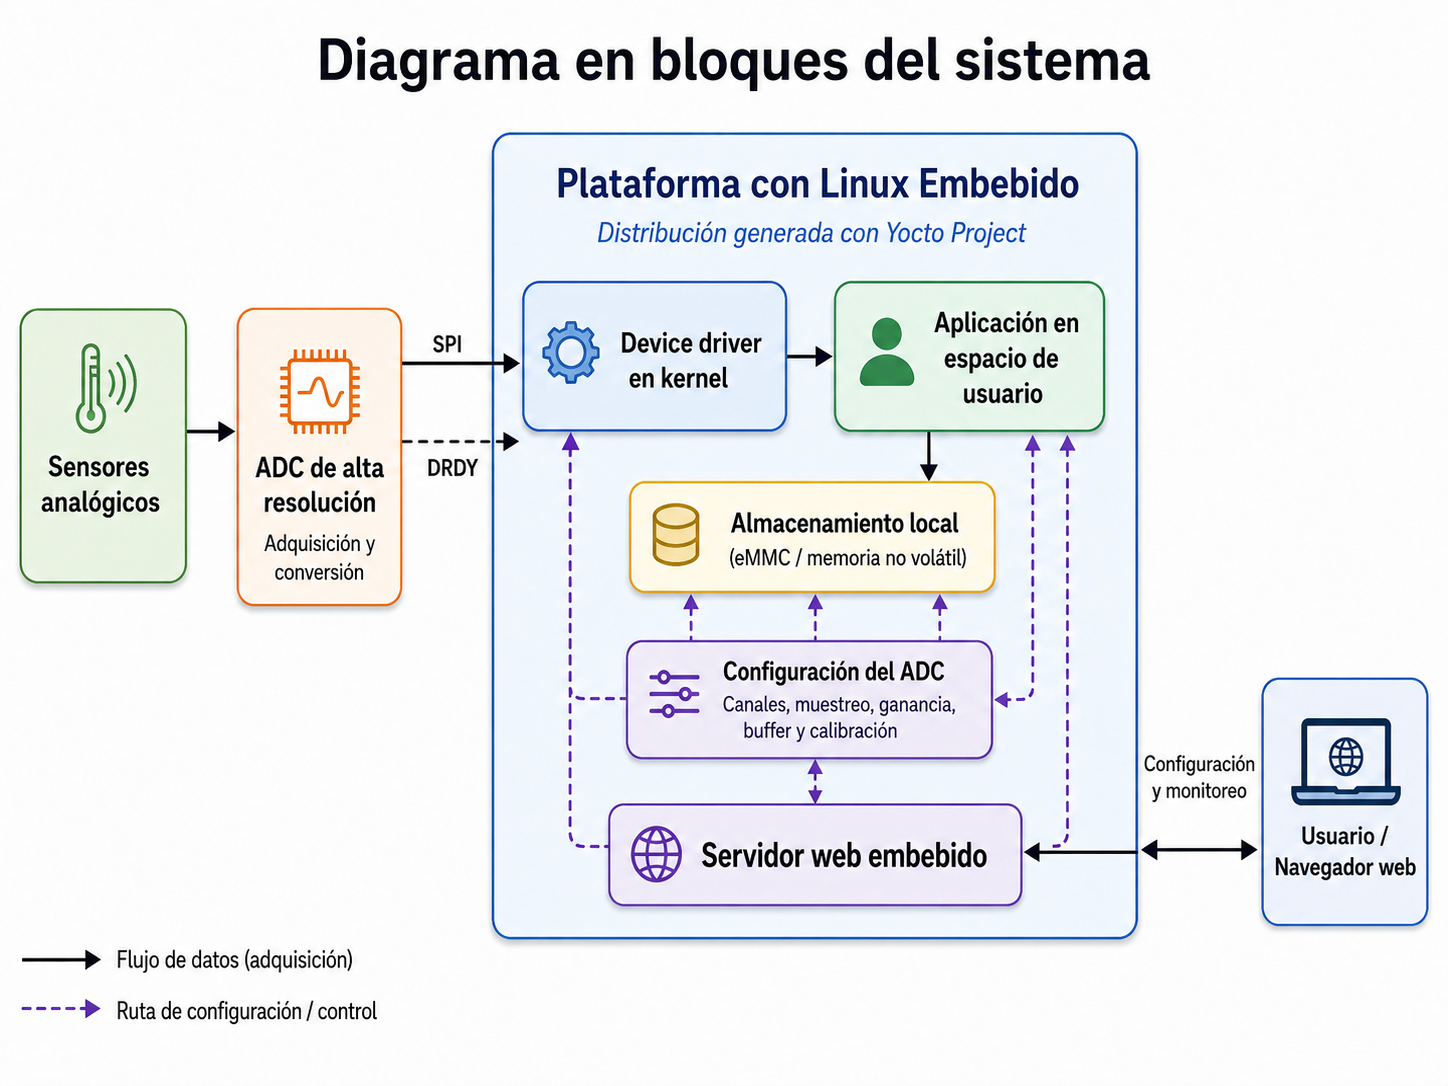
\includegraphics[width=0.95\textwidth]{Figuras/BlockDiagram.png}
    \caption{Diagrama en bloques del \textit{data logger} de alta velocidad basado en Linux embebido.}
    \label{fig:diagBloques}
\end{figure}

\FloatBarrier

La propuesta de valor del proyecto se centra en ofrecer una alternativa embebida, flexible y adaptable para la adquisición de datos de alta resolución, incorporando almacenamiento local, configuración dinámica y posibilidad de integración con sistemas de supervisión. El cliente objetivo corresponde a pequeñas y medianas industrias, integradores de automatización, laboratorios técnicos o áreas de mantenimiento que requieran registrar señales analógicas de forma confiable sin depender de soluciones cerradas, costosas o sobredimensionadas.

Los principales desafíos técnicos del proyecto se relacionan con la integración hardware-software, la configuración de una imagen de Linux embebido, la comunicación eficiente con el ADC, la reducción de latencias en el proceso de adquisición y la gestión del almacenamiento sin comprometer la continuidad del registro de datos. La innovación se encuentra en combinar un sistema Linux embebido personalizado, adquisición de datos a bajo nivel, almacenamiento local y configuración dinámica en una solución compacta orientada a escenarios industriales reales.

\section{2. Identificación y análisis de los interesados}
\label{sec:interesados}

\begin{table}[ht]
%\caption{Identificación de los interesados}
%\label{tab:interesados}
\begin{tabularx}{\linewidth}{@{}|l|X|X|l|@{}}
\hline
\rowcolor[HTML]{C0C0C0} 
Rol           & Nombre y Apellido & Organización 	& Puesto 	\\ \hline
Cliente       & \clientename      &\empclientename	& Líder del equipo de Investigación y Desarrollo \\ \hline
Responsable   & \authorname       & FIUBA        	& Alumno 	\\ \hline
\end{tabularx}
\end{table}

Las principales características de los interesados identificados son las siguientes:

\begin{itemize}
    \item Cliente: el Mg. Ing. Jonathan Cagua será quien evalúe y apruebe los resultados del proyecto. Asimismo, aportará orientación técnica durante el desarrollo del trabajo.
    
    \item Responsable: el Ing. Marcos Núñez será el encargado de planificar, diseñar, implementar, validar y documentar el prototipo propuesto.
\end{itemize}

\section{3. Propósito del proyecto}
\label{sec:proposito}

La realización de este trabajo responde a la necesidad de contar con una plataforma de adquisición de datos confiable, flexible y de bajo costo, orientada al registro de señales analógicas de alta velocidad mediante una solución embebida ajustada a los requerimientos del sistema. Mediante el uso de Yocto Project, se busca construir una distribución de Linux embebido a medida que permita adaptar el sistema operativo a las necesidades reales de una plataforma de adquisición de datos. De este modo, se pretende disminuir posibles fuentes de latencia durante la operación del dispositivo. Esta capacidad de construir una imagen específica para la aplicación resulta especialmente importante en un sistema de adquisición de alta velocidad, donde la continuidad del muestreo, la interacción eficiente con el hardware y la estabilidad del entorno de ejecución influyen directamente en la confiabilidad del registro de datos. En este contexto, el desarrollo de un \textit{device driver} integrado en el espacio de kernel permite gestionar la adquisición de datos con mayor eficiencia, menor latencia y mejor continuidad que una solución basada únicamente en aplicaciones de espacio de usuario. Con ello, el proyecto busca demostrar que es posible construir una solución de bajo costo, flexible y adaptable, capaz de cubrir necesidades de monitoreo e instrumentación que normalmente requieren equipos comerciales más costosos o menos modificables.


\section{4. Alcance del proyecto}
\label{sec:alcance}

El presente proyecto comprende el diseño, implementación y validación de un prototipo funcional de \textit{data logger} de alta velocidad basado en Linux embebido. El sistema estará orientado a la adquisición, procesamiento básico, almacenamiento y posterior disponibilidad de datos provenientes de señales analógicas, utilizando una plataforma embebida compatible con Linux y un convertidor analógico-digital de alta velocidad.

El alcance del proyecto se delimita en función de los componentes de hardware, software embebido, integración del sistema, pruebas funcionales y documentación técnica necesarios para demostrar la viabilidad de la solución propuesta.

El proyecto incluye:

\begin{itemize}
    \item Generación de una distribución personalizada de Linux embebido utilizando el meta-framework Yocto Project.

    \item Integración de la capa de soporte de hardware proporcionada por el fabricante, denominada \textit{Board Support Package} (BSP), para habilitar las características físicas del microprocesador STM32MP157D.

    \item Desarrollo e integración del driver de kernel para el convertidor analógico-digital ADS1256, incluyendo su declaración en el árbol de dispositivos (\textit{Device Tree}), la configuración de la interfaz SPI y la asignación de la señal DRDY como interrupción de sincronización para la adquisición de muestras.

    \item Implementación de funciones básicas de adquisición y configuración del ADC, tales como:
    \begin{itemize}
        \item selección de los canales de entrada;
        \item configuración de la frecuencia de muestreo disponible;
        \item ajuste de la ganancia programable;
        \item habilitación del buffer de entrada;
        \item rutinas básicas de calibración y control de conversión.
    \end{itemize}

    \item Implementación de lógicas operativas de almacenamiento para garantizar la escritura secuencial de las tramas adquiridas en soportes de memoria no volátil, utilizando serialización de datos binarios con el fin de reducir latencias asociadas a la manipulación de datos en formato ASCII.

    \item Verificación funcional del driver sobre la plataforma objetivo mediante pruebas de comunicación, configuración y adquisición de datos.

    \item Implementación de una interfaz web local mínima para parametrizar el sistema, limitada a:
    \begin{itemize}
        \item modificación de parámetros básicos de adquisición;
        \item consulta general del estado del dispositivo.
    \end{itemize}
\end{itemize}

El presente proyecto no incluye:

\begin{itemize}
    \item El diseño esquemático, el ruteo (\textit{PCB layout}) y la fabricación física de placas de circuito impreso dedicadas. El ecosistema físico se articulará mediante el ensamblaje y la instrumentación de prototipos, tarjetas de desarrollo comerciales o tarjetas de evaluación disponibles en el mercado que incluyan el SoC STM32MP157D y el periférico ADC ADS1256.

    \item La implementación de una aplicación compleja en espacio de usuario para registro continuo, almacenamiento masivo y gestión avanzada de archivos.

    \item La implementación de protocolos de comunicación industrial o de integración externa, tales como MQTT, SCADA o sockets TCP/UDP para supervisión remota.

    \item El diseño e implementación de filtros digitales complejos con coeficientes arbitrarios.

    \item El desarrollo de una interfaz web elaborada que incluya una experiencia de usuario avanzada, visualización histórica de datos o administración remota.

    \item La validación metrológica, certificación industrial o endurecimiento del producto para despliegue comercial.

    \item La incorporación del driver desarrollado al árbol principal del kernel Linux \textit{mainline} mediante un proceso formal de \textit{upstream}.
\end{itemize}

\section{5. Supuestos del proyecto}
\label{sec:supuestos}

Para el desarrollo del presente proyecto, se supone que existen las condiciones necesarias para diseñar, implementar y validar un \textit{data logger} de alta velocidad basado en Linux embebido. Dichos supuestos consideran la disponibilidad de recursos técnicos, humanos, materiales y organizacionales, así como la factibilidad de integración entre los distintos componentes del sistema. En particular, se establecen los siguientes supuestos:
\begin{itemize}
    \item Se dispone de una plataforma de desarrollo embebida compatible con Linux embebido, con soporte BSP vigente y con las interfaces de hardware necesarias para la adquisición, el almacenamiento local y la configuración del sistema;
    
    \item Se dispone del convertidor analógico-digital seleccionado, de su documentación técnica y de los elementos de interconexión requeridos para su integración con la plataforma de procesamiento;
    
    \item Existe compatibilidad eléctrica, lógica y temporal entre la plataforma embebida, el convertidor analógico-digital, el bus SPI, las señales de control e interrupción y el medio de almacenamiento empleado;
    
    \item La generación de una distribución de Linux embebido a medida mediante Yocto Project resulta técnicamente viable con los recursos de cómputo, la documentación disponible y el nivel de conocimiento alcanzable durante el desarrollo del trabajo;
    
    \item La integración del \textit{device driver} y de la configuración del \textit{device tree} en la imagen final del sistema es factible dentro del ecosistema de software seleccionado, sin requerir la incorporación del controlador al kernel Linux \textit{mainline};
    
    \item El nivel de desempeño alcanzable por la plataforma será suficiente para cumplir los objetivos de adquisición y registro definidos para el proyecto, manteniendo continuidad operativa y una latencia compatible con la aplicación prevista;
    
    \item Se dispone de las herramientas de desarrollo, depuración, medición e instrumentación necesarias para validar la comunicación con el periférico, la captura de muestras y la escritura de datos en memoria no volátil;
    
    \item Se cuenta con acceso a una red local o a un mecanismo equivalente de conexión que permita verificar la interfaz web mínima prevista para la configuración básica del sistema;
    
    \item Se dispone del tiempo de dedicación y de los recursos humanos necesarios para llevar adelante las tareas de integración, prueba, ajuste y documentación del prototipo;
    
    \item No se presentarán restricciones logísticas, reglamentarias o económicas extraordinarias que impidan la adquisición de componentes, el acceso a herramientas o la ejecución del proyecto dentro del período planificado.
\end{itemize}

\end{document}